\chapter{Measurement of Directional Characteristics II}\label{ax:directional_2}
This appendix serves as a protocol to a series of measurements conducted on the 2\textsuperscript{nd} of March 2018 in the large anechoic chamber (B4-111) at the acoustical lab of Aalborg University at Fredrik Bajers Vej 7.\\
The goal of these measurements was to quantify the directional characteristics of the loudspeakers that will be used in the loudspeaker array. The results are useful to show, what assumptions can be made when the speaker array is set up and where the position of the acoustic center is in relation to the cabinet. They will also serve as a baseline to which the directional characteristics of the speaker array can be compared. Furthermore, more experience can be gained regarding the practical aspects of measurement.

\section*{Measuring Equipment and Materials}
The following measuring equipment was used:
\begin{itemize}[noitemsep]
\item Microphone \gls{bandk} 4144
\begin{itemize}[noitemsep]
\item AAU-number: 06552
\item Serial number: 297090
\end{itemize}
\item Preamplifier GRAS 26AK
\begin{itemize}[noitemsep]
\item AAU-number: 56525
\item Serial number: 32811
\end{itemize}
\item Power supply \gls{bandk} 2804
\begin{itemize}
\item AAU-number: 06998
\item Serial number: 455309
\end{itemize}
\item Calibrator gls{bandk}\ 4231
\begin{itemize}[noitemsep]
\item AAU-number: 33691
\item Serial number: 2115338
\end{itemize}
\item Power Amplifier Pioneer A-616
\begin{itemize}[noitemsep]
\item AAU-number: 08249
\item Serial number: HJ9404841S
\end{itemize}
\item Sound card RME Fireface UCX
\begin{itemize}[noitemsep]
\item AAU-number: 108230
\item Serial number: 23811948
\end{itemize}
\item Turntable: Outline ET 250-3D
\begin{itemize}
\item Serial number: REIBO012
\end{itemize}
\item MATLAB r2017b on OSX 10.11.6
\item Loudspeaker SEAS 33 F-WKA
\end{itemize}

The following material was used:
\begin{itemize}[noitemsep]
%\item \SI{1/2}{\inch} to \SI{1}{\inch} preamp adapter
\item Microphone clip
\item Microphone stand
\item LEMU cable
\item XLR cable
\item Ethernet cable
\item Loudspeaker stand
\item Loudspeaker cabinet, plywood, outside dimensions: (400x400x400)\SI{}{\milli\meter}, wall~thickness:~\SI{20}{\milli\meter}
\item Speaker mount for turntable
\begin{itemize}[noitemsep]
\item Circular \gls{mdf} cutout, thickness: \SI{12}{\milli\meter}, {\(\varnothing\)~:~\SI{800}{\milli\meter}}
\item Top plate (\gls{mdf}), thickness: \SI{12}{\milli\meter}, surface : (400x400)\SI{}{\milli\meter}
\item 3 battens, (40x40x900)\SI{}{\milli\meter}
\item 3 aluminium brackets
\item 8 bolts M8x30, associated washers
\item miscellaneous woodscrews

\end{itemize}
\end{itemize}

\section*{Setup}
A sketch of the measurement setup can be found in \autoref{fig:measurement_setup}. A picture is given in \autoref{fig:setup_03_02}

\begin{figure}[htbp]
	\centering
	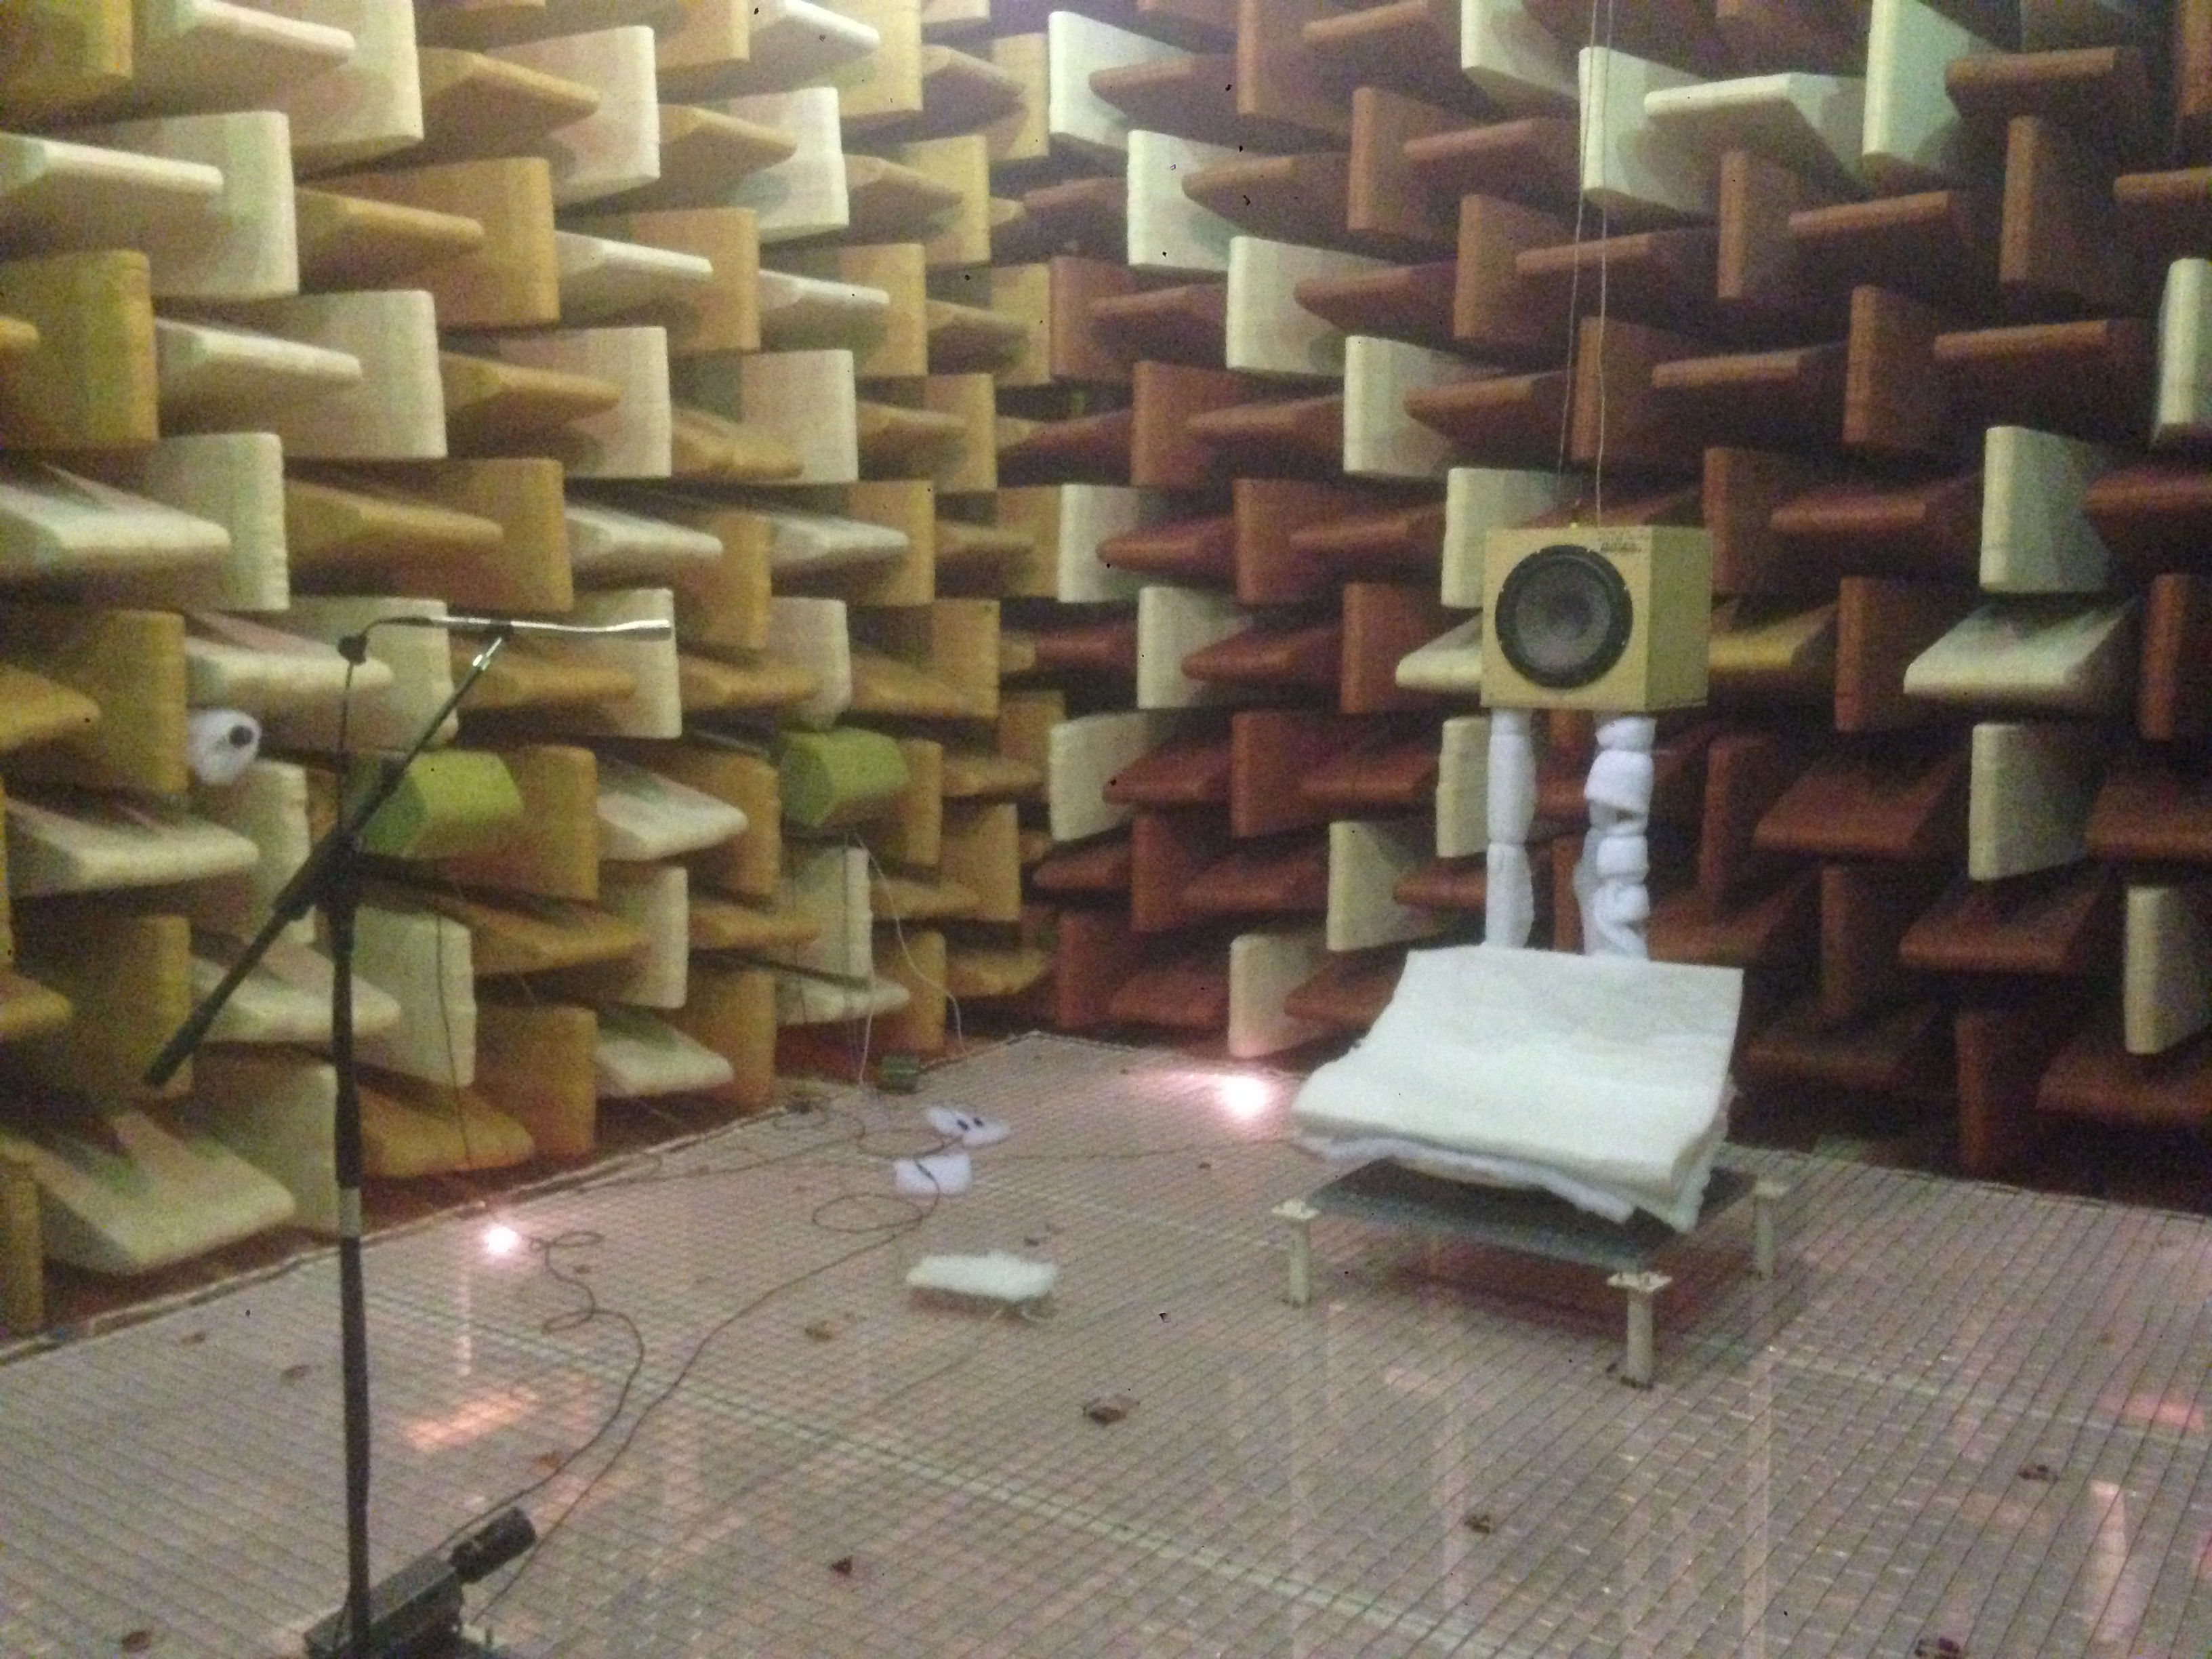
\includegraphics[width=0.7\textwidth]{03_02_setup.JPG}
	\caption{Measurement setup}
		\label{fig:setup_03_02}
\end{figure}

The horizontal distance between the microphone and the edge of the cabinet was \SI{2.74}{\meter}.